\chapter{Discussion}
\thispagestyle{fancy}
\label{sec:discussion}
\bigskip
%% \begin{table*}
% \caption{Average AUC values of approaches corresponding to prediction cases determined as multicollinear (VIF > 10, 5, 4, or 2.5) among the features selected by the WFS technique. We use decision tree for the machine learning algorithm. The $n$ in the last column is the number of prediction cases that contains multicollinearity among 1400 prediction cases.}
% \label{tab:comparingapproaches}
% \begin{tabular}{@{ }c@{ }|@{ }c@{ }|@{ }c@{ }|@{ }c@{ }|@{ }c@{ }|@{ }c@{ }|@{ }c@{ }|@{ }c@{ }|@{ }c@{ }|@{ }c@{ }|@{ }c@{ }}
% \hline

% \multicolumn{11}{c}{\bf AUC} \\ \cline{1-11}
% None & Default-PCA & NSVIF10 & NSVIF5 & NSVIF4 & NSVIF2.5 & SVIF10 & SVIF5 & SVIF4 & SVIF2.5 & WFS-BestFirst \\ \hline \hline

% 0.685&0.646&0.625&0.633&0.619&0.595&0.684&0.701&0.706&0.695&0.706 (n = 384, VIF > 10) \\ \hline
% 0.693&0.660&0.657&0.663&0.648&0.627&0.688&0.700&0.705&0.699&0.711 (n = 714, VIF > 5) \\ \hline
% 0.693&0.661&0.665&0.669&0.655&0.635&0.689&0.700&0.703&0.698&0.710 (n = 883, VIF > 4 )\\ \hline
% 0.693&0.663&0.673&0.675&0.662&0.640&0.692&0.700&0.703&0.700&0.711 (n = 1157, VIF > 2.5)\\ \hline 
% % \bf Average & 0.691& 0.658& 0.655& 0.660& 0.646& 0.624& 0.688& 0.700& 0.704& 0.698& 0.706& 0.710 \\ \hline 					
% \end{tabular}
% \end{table*}

% Please add the following required packages to your document preamble:
% \usepackage{graphicx}
\begin{table*}
\centering
\caption{Average AUC values of approaches corresponding to prediction cases determined as multicollinear (VIF > 10, 5, 4, or 2.5) in original dataset. We use decision tree for the machine learning algorithm. The $n$ in the last column is the number of prediction cases that contains multicollinearity among 4500 prediction cases.}
\label{tab:comparingapproaches_None}
\resizebox{\textwidth}{!}{%
\begin{tabular}{c|c|c|c|c|c|c|c|c|c|c|c}
\hline
\multicolumn{12}{c}{\textbf{AUC}} \\ \hline
\textbf{None} & \textbf{Default-PCA} & \textbf{NSVIF10} & \textbf{NSVIF5} & \textbf{NSVIF4} & \textbf{NSVIF2.5} & \textbf{SVIF10} & \textbf{SVIF5} & \textbf{SVIF4} & \textbf{SVIF2.5} & \textbf{VCRR} & \textbf{CFS} \\ \hline
\hline
0.662 (n = 4,102, VIF \textgreater 10)&  0.659&	0.654&	0.635&	0.633&	0.587&	0.661&	0.665&	0.666&	0.662&	0.665&	0.669  \\ \hline
0.664 (n = 4,400, VIF \textgreater 5) &	 0.658&	0.657&	0.639&	0.634&	0.593&	0.663&	0.667&	0.667&	0.661&	0.666&	0.671 \\ \hline
0.664 (n = 4,400, VIF \textgreater 4) &  0.658&	0.657&	0.639&	0.634&	0.593&	0.663&	0.667&	0.667&	0.661&	0.666&	0.671 \\ \hline
0.664 (n = 4,400, VIF \textgreater 2.5)& 0.658&	0.657&	0.639&	0.634&	0.593&	0.663&	0.667&	0.667&	0.661&	0.666&	0.671 \\ \hline
\end{tabular}%
}
\end{table*}

%We observed multicollinearity is not harmful the defect prediction performance. 
%  in Section~\ref{sec:result}. 
%To analyze our results in various aspects, we investigate following additional questions in this section.
% \begin{figure}[t]
% 	\centering
% 	\includegraphics[width=\linewidth]{figures/result/LR.png}
% 	\caption{Comparison of average ranks of considered approaches as regards mean AUC. Approaches for which the Nemenyi test results ($p =0.05$).
% 	% indicate that the differences are not significantly different are connected. 
% 	A logistic regression machine learning algorithm was used.}
% 	\label{fig:logistic_nemenyi}
% \end{figure}
% \begin{figure}[t]
% 	\centering
% 	\includegraphics[width=\linewidth]{figures/result/RF.png}
% 	\caption{Comparison of average ranks of considered approaches as regards mean AUC. Approaches for which the Nemenyi test results ($p =0.05$).
% 	% indicate that the differences are not significantly different are connected. 
% 	A random forest machine learning algorithm was used.}
% 	\label{fig:randomforest_nemenyi}
% \end{figure}

% \section{Performance with Various Classifiers}
% \label{subsecVariousClassifiers}
% We also conducted our experiments in which prediction models were constructed using logistic regression and random forest as a classifier. We evaluate the impact of multicollinearity when using other machine learners.
% We conducted the Friedman test with the Nemenyi test ($p<0.05$) to determine whether the rankings of the prediction models differed with statistical significance. 
% % Figure~\ref{fig:logistic_nemenyi} shows the comparisons of the average ranks of prediction model types obtained using logistic regression machine learners.
% Figures~\ref{fig:logistic_nemenyi} and~\ref{fig:randomforest_nemenyi} show the comparison of average ranks of the types of the models using logistic regression and random forest, respectively.
% % Figure~\ref{fig:logistic_nemenyi},~\ref{fig:randomforest_nemenyi}, and~\ref{fig:naivebayes_nemenyi} show the comparison of average ranks of the types of prediction models using the above three machine learners. 
% % \jc{Overall result, intepretations are too many to get the kye points. Summrize the key points that you want to sell the readers.}
% \subsection{Logistic regression}
% \label{logisticregression}
% When logistic regression was used as a classifier for building bug prediction models, 
% we found that the experimental result is similar to that of decision tree based bug prediction models. 
% In Figure~\ref{fig:logistic_nemenyi}, \emph{Default-PCA} had a higher average ranking than \emph{None}, at 4.089 and 4.133, respectively.
% % For example, the average ranking for \emph{None} is 4.844 while that of \emph{Default-PCA} is 5.067.
% However, \emph{Default-PCA} is connected to \emph{None}. Thus, the difference in ranking between \emph{Default-PCA} and \emph{None} is not statistically significant. 
% Moreover, there is no statistically significant difference (the Wilcoxon signed-rank test, $p<0.05$) between \emph{None} and \emph{Default-PCA} in terms of mean AUC of all 45 datasets. For the Cliff's delta effect size for prediction performance in terms of mean AUC all 45 datasets between \emph{PCA-Default} and \emph{None}, the difference magnitude is negligible. % ($|d|:0.041$). 
% Through three statistical methods, we found that the difference between \emph{Default-PCA} and \emph{None} for prediction performance is not significant. In terms of VIF and VCRR, we observed similar results, i.e., defect prediction models that used VIF or VCRR to remove multicollinearity do not significantly improve prediction performance compared to those of \emph{None}.
% %Thus, we conclude that PCA feature extraction technique does not have significant impact for better predictive performance
% %%VIF
% % To address RQ2, we first compare \emph{None} with \emph{SVIF5}, which has the best prediction performance among the approaches to which the VIF technique was applied in our experimental setup.
% % From Figure~\ref{fig:logistic_nemenyi},
% % \emph{None} had a higher average ranking than \emph{SVIF5}, at 4.844 and 5.044, respectively.
% % % For example, the average ranking for \emph{None} is 4.844 while that of \emph{SIVF5} is 5.044.
% % \emph{None} and \emph{SVIF5} are connected by the same line, indicating that no statistically significant difference in ranking was indicate by the Nemenyi post-hoc test. Moreover, there is no statistically significant difference (the Wilcoxon signed-rank test, $p<0.05$) between \emph{None} and \emph{SVIF5} in terms of mean AUC for all 45 datasets. For the Cliff's delta effect size for prediction performance in terms of mean AUC all 45 datasets between \emph{SVIF5} and \emph{None}, the difference magnitude is negligible.
% % Through three statistical methods, we found that the difference between \emph{SVIF5} and \emph{None} for prediction performance was not significant. Thus, we conclude that the VIF feature selection technique does not significantly improve prediction performance.
% %%%VCRR
% % To address RQ3, we compare \emph{None} with \emph{VCRR}. In Figure~\ref{fig:logistic_nemenyi}, 
% % \emph{None} has a higher average ranking than \emph{VCRR}, at 4.844 and 6.355, respectively. \emph{None} and \emph{VCRR} are connected to the same line, indicating that no statistically significant difference in ranking was indicate by the Nemenyi post-hoc test. Moreover, there is no statistically significant difference (the Wilcoxon signed-rank test, $p<0.05$) between \emph{None} and \emph{VCRR} in terms of mean AUC for all 45 datasets. For the Cliff's delta effect size for prediction performance in terms of mean AUC all 45 datasets between \emph{VCRR} and \emph{None}, the difference magnitude is negligible.
% % Through three statistical methods, we found that the difference between \emph{VCRR} and \emph{None} for prediction performance was not significant. Thus, we conclude that the variable clustering and removal of redundant metrics does not have significant impact for better predictive performance.
% Our experimental result shows that it is difficult to state that multicollinearity removal method (i.e., PCA, VIF, and VCRR) can yield superior prediction results with statistical significance. Therefore, we conclude that multicollinearity is not particularly harmful to defect prediction models when using logistic regression.

% \subsection{Random forest}
% \label{randomforest}
% When building bug prediction models with random forest, we also observed that the experiment results are 
% similar to that of bug prediction models built with decision tree.
% %To address RQ1, we compare \emph{None} with \emph{Default-PCA}.
% In Figure~\ref{fig:randomforest_nemenyi}, \emph{None} had a higher average ranking than \emph{Default-PCA}, at 2.777 and 6.600, respectively.
% % For example, the average ranking for \emph{None} is 4.844 while that of \emph{Default-PCA} is 5.067.
% Moreover, \emph{Default-PCA} is not connected to \emph{None}. Thus, the difference in ranking between \emph{Default-PCA} and \emph{None} is statistically significant. There is also statistically significant difference (the Wilcoxon signed-rank test, $p<0.05$) between \emph{None} and \emph{Default-PCA} in terms of mean AUC of all 45 datasets. For the Cliff's delta effect size for prediction performance in terms of mean AUC all 45 datasets between \emph{PCA-Default} and \emph{None}, the difference magnitude is small. 
% Through three statistical methods, we found that the difference between \emph{Default-PCA} and \emph{None} for prediction performance is significant. 
% Thus, we conclude that PCA feature extraction technique has a negative impact on predictive performance when using random forest. 
% In terms of VIF and VCRR, we also could not observe the positive impact on prediction performance compared to \emph{None} when using random forest.


%%VIF
% To address RQ2, we first compare \emph{None} with \emph{SVIF10}, which has the best prediction performance among the approaches to which the VIF technique was applied in our experimental setup.
% From Figure~\ref{fig:randomforest_nemenyi},
% \emph{None} had a higher average ranking than \emph{SVIF10}, at 2.777 and 3.022, respectively.
% % For example, the average ranking for \emph{None} is 4.844 while that of \emph{SIVF5} is 5.044.
% \emph{None} and \emph{SVIF10} are connected by the same line, indicating that no statistically significant difference in ranking was indicate by the Nemenyi post-hoc test. Moreover, there is no statistically significant difference (the Wilcoxon signed-rank test, $p<0.05$) between \emph{None} and \emph{SVIF10} in terms of mean AUC for all 45 datasets. For the Cliff's delta effect size for prediction performance in terms of mean AUC all 45 datasets between \emph{SVIF10} and \emph{None}, the difference magnitude is negligible.
% Through three statistical methods, we found that the difference between \emph{SVIF10} and \emph{None} for prediction performance is not significant. Thus, we conclude that the VIF feature selection technique does not significantly improve prediction performance.

%%%VCRR
% To address RQ3, we compare \emph{None} with \emph{VCRR}. In Figure~\ref{fig:randomforest_nemenyi}, 
% \emph{None} has a higher average ranking than \emph{VCRR}, at 2.777 and 5.155, respectively. \emph{None} and \emph{VCRR} are not connected to the same line, indicating that statistically significant difference in ranking was indicate by the Nemenyi post-hoc test. Moreover, there is statistically significant difference (the Wilcoxon signed-rank test, $p<0.05$) between \emph{None} and \emph{VCRR} in terms of mean AUC for all 45 datasets. For the Cliff's delta effect size for prediction performance in terms of mean AUC all 45 datasets between \emph{VCRR} and \emph{None}, the difference magnitude is negligible.
% Through three statistical methods, we found that the difference between \emph{VCRR} and \emph{None} for prediction performance was significant. Thus, we conclude that the variable clustering and removal of redundant metrics has significant impact for worse predictive performance.

%Our experimental result shows that it is difficult to state that multicollinearity removal method (i.e., PCA, VIF, and VCRR) can yield superior prediction results with statistical significance. Therefore, we conclude that multicollinearity is not particularly harmful to defect prediction models when using random forest.


In this section, we analyze interesting observations more and discuss implications of the findings and threats to validity.
\section{ SVIF and NSVIF results}
\label{secSVIF}
% \jc{why do you want to discuss this point. Explain it first.}
% among the VIF approaches such as \emph{NSVIF10}, \emph{NSVIF5}, \emph{NSVIF4}, \emph{NSVIF2.5}, and \emph{SVIF10} is lower ranking than \emph{None}.

We observed that the performance achieved using NSVIF is most likely inferior to that obtained with SVIF in our experiments, although both techniques remove multicollinearity.
% For example, in Figure~\ref{fig:baselines_decisiontree_nemenyi}, \emph{SVIF5}, \emph{SVIF4}, \emph{SVIF2.5}, and \emph{CFS-BestFirst} have the higher rankings of the average AUC than those of \emph{None}. 
% On the other hand, \emph{NSVIF10}, \emph{SVIF10}, \emph{NSVIF5}, \emph{Default-PCA}, \emph{NSVIF4}, and \emph{NSVIF2.5} have the lower rankings of the average AUC than those of \emph{None}.
For example, in Table~\ref{tab:baselinesofresults}, all SVIF models have higher the mean AUC than all NSVIF models. 
In Section~\ref{sec:result}-RQ2, the \emph{None} ranked highest, followed by \emph{SVIF10}, \emph{SVIF5}, and \emph{SVIF4}. In addition, in Section~\ref{sec:result}-RQ3, \emph{SVIF4} and \emph{SVIF10}, respectively, were ranked first for decision tree model and random forest model. Also, in all machine learners, NSVIF models were ranked low in common. 
When conducting the Wilcoxon signed-rank test, the number of significantly lower-performance models than \emph{None} was 2 out of 30 for \emph{SVIF10} and 27 for \emph{NSVIF2.5} and \emph{NSVIF5} (in case `B').
% In Figure~\ref{fig:baselines_decisiontree_nemenyi}, there are some approaches applying NSVIF (i.e., \emph{NSVIF10}, \emph{NSVIF5}, \emph{NSVIF4}, and \emph{NSVIF2.5}) have lower rankings than \emph{None}. 
% In addition, \emph{SVIF4} are not connected by the same line with \emph{NSVIF2.4} and \emph{NSVIF4}. Thus, there is a difference with statistical significance in ranking by the Nemenyi post-hoc test.
% We also observed, in Table~\ref{tab:comparingapproaches_None}, all NSVIF approaches have a lower average AUC than \emph{None} with statical significance by the Wilcoxon signed-rank test ($p<0.05$). However, \emph{SVIF4} have the statistically significant difference compared to \emph{None} (the Wilcoxon signed-rank test, $p<0.05$).
% In Table~\ref{tab:comparingapproaches_CFS}, we observed there are all NSVIF approaches have a lower average AUC than \emph{None} with statical significance by the Wilcoxon signed-rank test ($p<0.05$). 

To better understand our results in terms of the VIF, we investigated the factors that affect the prediction performance by considering the differences between SVIF and NSVIF.
% We want to explore how leaving informative features behind through the differences between Stepwise VIF (SVIF) and Non-Stepwise VIF (NSVIF) affects predictive performance.
The main difference between the two techniques is the application of stepwise techniques. NSVIF calculates the VIF once only and removes all features with VIF values exceeding a certain threshold. However, SVIF does not delete all features for which the VIF values exceed the threshold; instead, only the feature having the largest VIF value is removed following each VIF calculation. This difference shows that retention of informative features can have a positive performance impact. The risk of removing features that have strongly impact the dependent variable is greater in NSVIF than in SVIF. This is because NSVIF removes many features that exceed the threshold at the same time. However, SVIF omits one feature at a time. Recalculating VIF for the remaining features may decrease their VIF values of the features removed in NSVIF. Therefore, retaining informative features could be an effective means of improving prediction performance, rather than removal of multicollinearity. These results imply that we should be careful when applying multicollinearity removal techniques for defect prediction studies.

%\section{Explanation of boxplot results}
%\label{subsecBoxplot}
\begin{figure}[t]
	\centering
	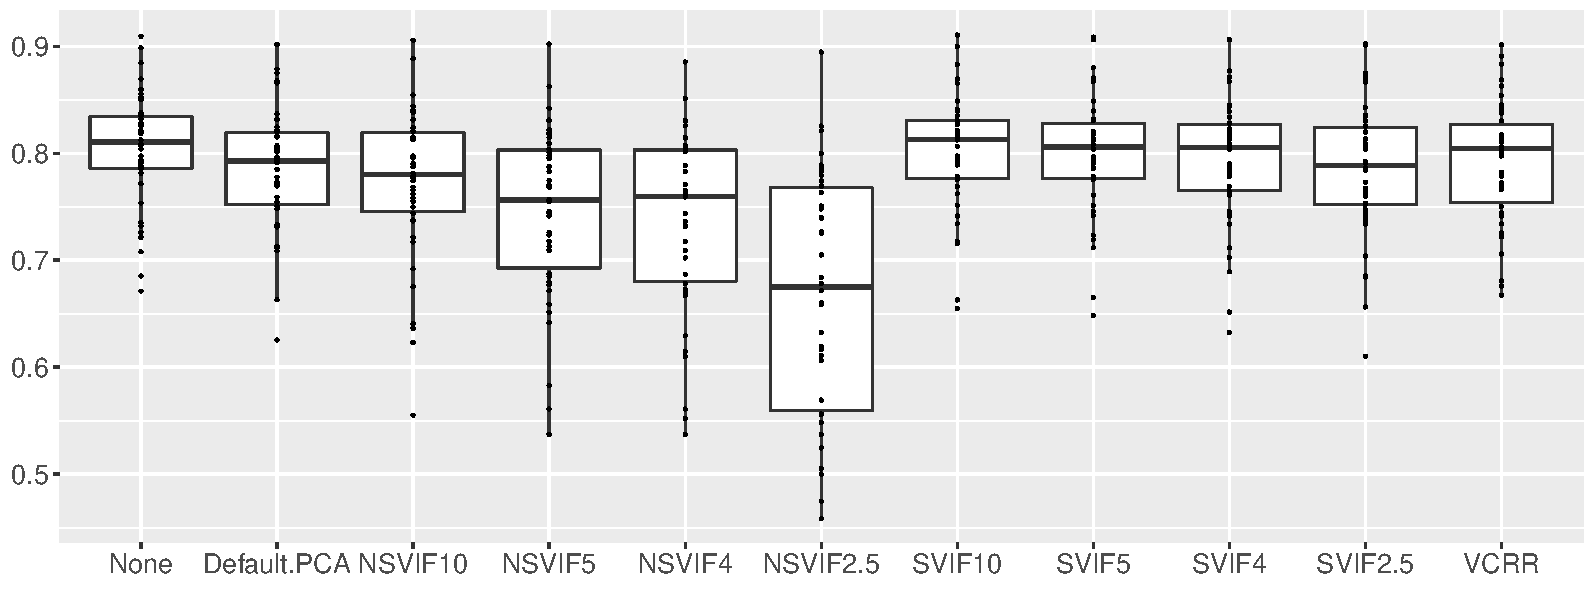
\includegraphics[width=1\linewidth]{pdfs/RF_1_AUC_5_multicollinearity_with_None_thres_10.0_6_average.csv_boxplot.pdf}
	\caption{Boxplot of the average AUC value of 11 models with respect to 45 dataset with multicollinearity (`B' case). A random forest machine learning algorithm was used.}
	\label{fig:boxplot_RF_AUC_B_case}
\end{figure}

Figure~\ref{fig:boxplot_RF_AUC_B_case} shows a boxplot from the results of the random forest model in Table~\ref{tab:baselinesofresults}. As the random forest model leads to the highest AUC performance, we present this as a representative result to show the boxplot. 
% \footnote{The entire boxplots will be shared as an online appendix after the blind review.} 
We found that compared to \emph{None}, the difference between the first and third quartiles of \emph{NSVIF2.5} is particularly large. This is a large deviation of the data, and the results will be interpreted as unstable. 
We can also see in NVIF models that the smaller the threshold, the greater the deviation. In SVIF models, on the other hand, the deviations do not vary significantly depending on the threshold.
As described in Section~\ref{sec:discussion}-\ref{secSVIF}, this is because NVIF models delete metrics that have multicollinearity at once. As multicollinearity is more strictly removed, significant metrics will be deleted, resulting in lower performance. This may result in less stable results in comparison of prediction performance or analysis of performance if multicollinearity is removed in the defect prediction study.

% \section{Are the original datasets suffering from multicollinearity problem?}
% \label{subsecCheckMulticollinearityNone}
% We examined the multicollinearity of the original dataset to correctly investigate the effects of multicollinearity. If the original dataset did not suffer from multicollinearity, the effects of removing multicollinearity technique would not be significant and this could affect the interpretation of our experimental results. To check the multicollinearity, we used a VIF with a threshold value of 10, a commonly used threshold value suggested by Gujarati~\cite{gujarati2009basic}. 
% In \emph{None} models, we found that 91.16\%  of models (4,102 out of 4,500 cases) have the multicollinearity issue.

% Although many cases have suffered from multicollinearity, to accurately analyze the effects of multicollinearity on predictive performance, we conducted our experiments again only with the models that suffer from the multicollinearity issue.
% % compare the performance of datasets determined to have multicollinearity
% We first found the datasets determined as multicollinearity on the original dataset from Table~\ref{tab:baselinesofresults}. Since various VIF thresholds were considered in the experiments reported in Section~\ref{sec:experimentalsetup}, we used VIFs with various threshold values, i.e., 10, 5, 4, and 2.5, to check for multicollinearity. Table~\ref{tab:comparingapproaches_None} lists the average AUC values of prediction models based on the 11 considered model types corresponding to the datasets.
% % \jc{put None column as the first column and CFS column as a last column in Table 4} 

% In Table~\ref{tab:comparingapproaches_None}, we found that \emph{SVIF4}, \emph{SVIF5}, and \emph{VCRR} have a higher performance than \emph{None} in average AUC. 
% However, \emph{Default-PCA}, \emph{NSVIF10}, \emph{NSVIF5}, \emph{NSVIF4}, \emph{NSVIF2.5}, \emph{SVIF10}, and \emph{SVIF2.5} have lower performance than \emph{None}.
% \emph{SVIF4} has the statistically significant difference compared to \emph{None} (the Wilcoxon signed-rank test, $p<0.05$) among the higher performance models than \emph{None}. 
% In addition, \emph{PCA}, \emph{NSVIF10}, \emph{NSVIF5}, \emph{NSVIF4}, \emph{NSVIF2.5} have the statistically significant difference compared to \emph{None} (the Wilcoxon signed-rank test, $p<0.05$) among the lower performance models than \emph{None}. As a result, we conclude that, with the exception of \emph{SVIF4}, techniques that remove multicollinearity (e.g., \emph{Default-PCA}, \emph{SVIF10}, \emph{SVIF5}, \emph{SIVF2.5}, \emph{VCRR}, and all NSVIF approaches) do not have significant impact on better predictive performance. Even, \emph{Default-PCA} and all NSVIF approaches decrease the performance of prediction model. 
% (The CFS column will be discussed in Section~\ref{subsec:cfs}.)

\section{ Does applying a widely used feature selection have positive impact on performance?}
\label{subsec:cfs}
From our survey in Section~\ref{sec:background}-\ref{sec:survey}, we found that techniques removing multicollinearity were also used as a feature selection technique. Generally, feature selection is known as a necessary preprocessing step to improve prediction models. In this sense, investigating prediction performance in the view of feature selection is important to show removing multicollinearity has a different purpose from feature selection.
%As in Section~\ref{sec:result}, we concluded that removing multicollinearity does not have significant impact on prediction performance.

Thus, we conducted additional experiments if a widely used feature selection approach can impact on prediction performance under our experimental setting. We compared the models of \emph{None} to those based on a representative feature selection approach, i.e., the Correlation-based feature selection technique (CFS)~\cite{Hall99correlation-basedfeature}. CFS is known as one of the best feature selection methods for defect prediction models~\cite{ghotra2017msr}. In our experiments, we used best-first searching as a heuristic search strategy for CFS, as in Ghotra et al.~\cite{ghotra2017msr}. 
% Note that \emph{CFS does not perfectly remove the multicollinearity, but it only does its best to select features, which are more related with the class (i.e. response variable) and less related with other features in the selected feature group}.
% \jc{could we cite Hassans paper as well?}.
%In addition, we add the Correlation-based feature selection technique~\cite{Hall99correlation-basedfeature} as a new approach in our experiment. Previous studies recommended the CFS to improve defect prediction performance~. Thus, we added the CFS as a new approach in our experiment to compare performance with multicollinearity removal techniques.
% Please add the following required packages to your document preamble:
% \usepackage{multirow}
% \usepackage{graphicx}
\begin{table}[t!]
\centering
\caption{Comparison of results between None and CFS models in terms of a mean value for 45 datasets}
\label{tab:CFS}
\resizebox*{!}{0.9\textheight}{%
\begin{tabular}{|c|c|c|c|c|}
\hline
\textbf{ML} & \textbf{Measurement} & \textbf{\# of prediction cases} & \textbf{None} & \textbf{CFS} \\ \hline
\multirow{10}{*}{LR}  & \multirow{2}{*}{AUC}       & A & 0.746 & 0.750(N)                    \\ \cline{3-5} 
                      &                            & B & 0.743 & 0.773(N)                   \\ \cline{2-5} 
                      & \multirow{2}{*}{Precision} & A & 0.640  & 0.636(N)                   \\ \cline{3-5} 
                      &                            & B & 0.625 & 0.684(N)                   \\ \cline{2-5} 
                      & \multirow{2}{*}{Recall}    & A & 0.466 & 0.422*(N)                  \\ \cline{3-5} 
                      &                            & B & 0.488 & 0.472*(N)                  \\ \cline{2-5} 
                      & \multirow{2}{*}{Fmeasure}  & A & 0.506 & 0.476*(N)                  \\ \cline{3-5} 
                      &                            & B & 0.524 & 0.539\textasciicircum{}(N) \\ \cline{2-5} 
                      & \multirow{2}{*}{MCC}       & A & 0.318 & 0.296*(N)                  \\ \cline{3-5} 
                      &                            & B & 0.316 & 0.359(N)                   \\ \hline
\multirow{10}{*}{DT}  & \multirow{2}{*}{AUC}       & A & 0.664 & 0.670(N)                    \\ \cline{3-5} 
                      &                            & B & 0.650  & 0.666\textasciicircum{}(N) \\ \cline{2-5} 
                      & \multirow{2}{*}{Precision} & A & 0.592 & 0.611\textasciicircum{}(N) \\ \cline{3-5} 
                      &                            & B & 0.588 & 0.651(N)                   \\ \cline{2-5} 
                      & \multirow{2}{*}{Recall}    & A & 0.494 & 0.465(N)                   \\ \cline{3-5} 
                      &                            & B & 0.517 & 0.496(N)                   \\ \cline{2-5} 
                      & \multirow{2}{*}{Fmeasure}  & A & 0.522 & 0.502(N)                   \\ \cline{3-5} 
                      &                            & B & 0.536 & 0.553(N)                   \\ \cline{2-5} 
                      & \multirow{2}{*}{MCC}       & A & 0.313 & 0.303(N)                   \\ \cline{3-5} 
                      &                            & B & 0.309 & 0.346(N)                   \\ \hline
\multirow{10}{*}{RF}  & \multirow{2}{*}{AUC}       & A & 0.803 & 0.772*(S)                  \\ \cline{3-5} 
                      &                            & B & 0.789 & 0.778*(S)                  \\ \cline{2-5} 
                      & \multirow{2}{*}{Precision} & A & 0.668 & 0.625*(S)                  \\ \cline{3-5} 
                      &                            & B & 0.647 & 0.665\textasciicircum{}(N) \\ \cline{2-5} 
                      & \multirow{2}{*}{Recall}    & A & 0.513 & 0.505*(N)                  \\ \cline{3-5} 
                      &                            & B & 0.527 & 0.527(N)                   \\ \cline{2-5} 
                      & \multirow{2}{*}{Fmeasure}  & A & 0.555 & 0.537*(N)                  \\ \cline{3-5} 
                      &                            & B & 0.559 & 0.569\textasciicircum{}(N) \\ \cline{2-5} 
                      & \multirow{2}{*}{MCC}       & A & 0.379 & 0.345*(N)                  \\ \cline{3-5} 
                      &                            & B & 0.366 & 0.375\textasciicircum{}(N) \\ \hline
\multirow{10}{*}{NB}  & \multirow{2}{*}{AUC}       & A & 0.738 & 0.739(N)                   \\ \cline{3-5} 
                      &                            & B & 0.729 & 0.762(N)                   \\ \cline{2-5} 
                      & \multirow{2}{*}{Precision} & A & 0.565 & 0.600\textasciicircum{}(N)   \\ \cline{3-5} 
                      &                            & B & 0.588 & 0.650\textasciicircum{}(N)  \\ \cline{2-5} 
                      & \multirow{2}{*}{Recall}    & A & 0.518 & 0.457*(N)                  \\ \cline{3-5} 
                      &                            & B & 0.450  & 0.475\textasciicircum{}(N) \\ \cline{2-5} 
                      & \multirow{2}{*}{Fmeasure}  & A & 0.490  & 0.484(N)                   \\ \cline{3-5} 
                      &                            & B & 0.488 & 0.527(N)                   \\ \cline{2-5} 
                      & \multirow{2}{*}{MCC}       & A & 0.287 & 0.302(N)                   \\ \cline{3-5} 
                      &                            & B & 0.285 & 0.352\textasciicircum{}(N) \\ \hline
\multirow{10}{*}{BN}  & \multirow{2}{*}{AUC}       & A & 0.754 & 0.752(N)                   \\ \cline{3-5} 
                      &                            & B & 0.743 & 0.765(N)                   \\ \cline{2-5} 
                      & \multirow{2}{*}{Precision} & A & 0.552 & 0.563\textasciicircum{}(N) \\ \cline{3-5} 
                      &                            & B & 0.566 & 0.599(N)                   \\ \cline{2-5} 
                      & \multirow{2}{*}{Recall}    & A & 0.572 & 0.563(N)                   \\ \cline{3-5} 
                      &                            & B & 0.578 & 0.601(N)                   \\ \cline{2-5} 
                      & \multirow{2}{*}{Fmeasure}  & A & 0.539 & 0.546(N)                   \\ \cline{3-5} 
                      &                            & B & 0.560  & 0.586(N)                   \\ \cline{2-5} 
                      & \multirow{2}{*}{MCC}       & A & 0.333 & 0.339(N)                   \\ \cline{3-5} 
                      &                            & B & 0.337 & 0.377(N)                   \\ \hline
\multirow{10}{*}{LMT} & \multirow{2}{*}{AUC}       & A & 0.760  & 0.751*(N)                  \\ \cline{3-5} 
                      &                            & B & 0.740  & 0.765(N)                   \\ \cline{2-5} 
                      & \multirow{2}{*}{Precision} & A & 0.665 & 0.659(N)                   \\ \cline{3-5} 
                      &                            & B & 0.644 & 0.695(N)                   \\ \cline{2-5} 
                      & \multirow{2}{*}{Recall}    & A & 0.454 & 0.439*(N)                  \\ \cline{3-5} 
                      &                            & B & 0.467 & 0.472(N)                   \\ \cline{2-5} 
                      & \multirow{2}{*}{Fmeasure}  & A & 0.513 & 0.501(N)                   \\ \cline{3-5} 
                      &                            & B & 0.515 & 0.545(N)                   \\ \cline{2-5} 
                      & \multirow{2}{*}{MCC}       & A & 0.333 & 0.322*(N)                  \\ \cline{3-5} 
                      &                            & B & 0.321 & 0.365(N)                   \\ \hline
\end{tabular}%
}
\end{table}

Table~\ref{tab:CFS} lists the performance of the defect prediction model and presents the results from machine learning classifiers in five measures. There are `A' and `B' in the column `\# of prediction cases'. `A' represents reporting the average value of all 4,500 predictions by 10 $\times$ 10 cross-validation of 45 project datasets. `B' indicates reporting the average value of the prediction cases corresponding to the data (2,164 predictions) in which multicollinearity problem was found when using the VIF technique with the threshold of 10 in the \emph{CFS}. 
We conduct the Wilcoxon signed-rank ($p<0.05$) and Cliff's $\delta$ tests at the average level to verify that each approach differs significantly from the \emph{None}. In Wilcoxon signed-rank test, approaches with significantly lower performance than \emph{None} are marked with an asterisk (*) and higher are marked with a caret (\textasciicircum{}). In the Cliff's $\delta$ test, the magnitude of the difference with \emph{None} such as negligible, small, medium, and large are marked as (N), (S), (M), and (L), respectively.

In Table~\ref{tab:CFS}, there are 9 prediction results in which \emph{CFS} perform better than \emph{None} and 21 prediction results in which the \emph{None} is higher. When conducting the Wilcoxon signed-rank test, there are 3 results where \emph{CFS} is significantly higher than \emph{None} and 12 results where \emph{None} is significantly higher than \emph{CFS}. 
However, there were no approaches to remove multicollinearity, which was significantly better performing than \emph{None} in Table~\ref{tab:baselinesofresults}.
 
The CFS technique does not perfectly remove the multicollinearity, but it only does its best to select features, which are more related with the class (i.e. response variable) and less related with other features in the selected feature group~\cite{Hall99correlation-basedfeature}. However, someone may think the reason why \emph{CFS} yields better results because of a low multicollinearity ratio; therefore, it was necessary to clarify this aspect. We computed the average values obtained from the prediction models constructed on datasets still having multicollinear features, which were selected through the CFS technique (Case `B'). We found the CFS-selected features are still multicollinear in 48.09\% (2,164 out of 4,500 cases) using VIF with 10.  Application of CFS to remove multicollinearity may be unsuccessful, because the CFS technique heuristically removes multicollinearity and its main purpose is to select informative features.

In case `B' of Table~\ref{tab:CFS}, there are 26 prediction results in which \emph{CFS} perform better than \emph{None} and 3 prediction results in which the \emph{None} was higher. When conducting the Wilcoxon signed-rank test, there are 8 results where \emph{CFS} is significantly higher than \emph{None} and 2 results where \emph{None} is significantly higher than \emph{CFS}. As a result, we conclude that the positive performance impact of the CFS technique is not related to multicollinearity. 

%\section{Are the selected features by CFS multicollinear?}
%\label{subsecCheckMulticollinearityCFS}
%To investigate further about the performance impact of multicollinearity, we analyzed whether selected features by CFS are multicollinear.
%We found that \emph{CFS} had the best performance in the experiment of Section~\ref{subsecCheckMulticollinearityNone}.
% Moreover, although \emph{WFS-BestFirst} has a lower average AUC than \emph{CFS-BestFirst}, there is no statistically significant difference between the two models (the Wilcoxon signed-rank test, $p<0.05$). 
The CFS technique chooses features considering the high correlation between the feature values and class labels. This is one possible reason why CFS yield better prediction performance; this result also confirm the findings of previous studies that the CFS techniques effectively improve prediction performance~\cite{ghotra2017msr}.
% Therefore, we infer the conclusion that the best performance of \emph{CFS-BestFirst} is not resulted to removing multicollinearity, but from selecting informative features. 
Hence, we infer that \emph{CFS} yields the best performance through selection of informative features rather than multicollinearity removal.

\section{ Implications and Guidelines}
\label{subsecPracticalGuideline}
\emph{Consider the research objectives first before treating the multicollinearity.}
% \textbf{Think about the research objectives first to deal with multicollinearity.}
% \jc{do not use `you' `yours'. Explain generally and objectively. you forgot to address this comment.}
When conducting a defect prediction study, we must consider whether our research goal is to analyze the impact of metrics or to improve the predictive performance. This is because it is necessary to remove multicollinearity for the former, but it is not necessary for the latter. However, as in our survey, some existing studies blindly removed multicollinearity for predicative performance. This is a misconception we have to avoid in defect prediction studies.

\emph{When analyzing the impact of metrics, multicollinearity must be removed.}
% \subsection*{When analyzing the impact of metrics, multicollinearity must to be removed.}
% \textbf{When analyzing the impact of metrics, multicollinearity needs to be removed.}
% \jc{put this as a second guideline. Try to follow the order of steps.)}
In Section~\ref{sec:background}-\ref{mathematicalreason}, we explained why multicollinearity is problematic from a mathematical perspective. Multicollinearity poses risks to statistical or data-mining analyses.
% First, it affects the precision of the estimated coefficients of the explanatory variables because it inflates the variance of the former.
% Second, it is that the estimation is unstable because the estimation results are very sensitive to changes in the dataset (even if the change is very small).
% Thus, we recommend multicollinearity need to be removed when analyzing metrics.
Thus, we recommend multicollinearity removal when analyzing the impact of metrics. %\jc{recommending implies optional. Use proper expressions.}

% We propose the following practical guidelines for defect prediction model construction. 
% Based on the theoretical background and empirical study, we suggest the following guidelines about the multicollinearity issue.
% \subsection*{Consider the research objectives first before treating the multicollinearity.}

\emph{It is not necessary to remove multicollinearity to improve prediction model performance.}
% \subsection*{It is not necessary to remove multicollinearity to improve prediction model performance.}
% \textbf{It is not necessary to remove multicollinearity to improve performance of prediction models.}
% We observed that SVIF performs better than NSVIF over all four prediction models. \jc{why is this the supporting points for the guideline 2?} 
% This observation can show that multicollinearity does not affect performance of defect prediction, as discussed in Section~\ref{subsecSVIF}. 
We found that multicollinearity and defect prediction performance are not significantly related. %, as discussed in Section~\ref{subsecCheckMulticollinearityNone}. % and~\ref{subsec:cfs}.
Our experimental results show that widely used multicollinearity removal methods (i.e. PCA, VIF, and VCRR) do not have a significant impact on better predictive performance. For example, in Section~\ref{sec:result}-RQ2, we observed none of the prediction results perform significantly better than \emph{None}. We even found that many models were worse than the \emph{None} with statistical significance. 
% we observed that PCA technique considering multicollinearity does not improve predictive performance because the ranking of \emph{Default-PCA} and \emph{None} are not statistically significant (the Nemenyi test, at $p = 0.05$). 
% Moreover, through RQ2, we observed that \emph{SVIF4} among the VIF approaches considering multicollinearity does not improve predictive performance because the ranking of \emph{SVIF4} and \emph{None} are not statistically significant (the Nemenyi test, at $p = 0.05$). 
% Therefore, we cannot conclude that removing multicollinearity improves performance. 
% Conversely, we cannot conclude that even if the prediction model has multicollinearity, the performance will be decreased. 
This finding coincides with the discussion in Section~\ref{sec:background}-\ref{predictionofmulticollinearity}. As reported in Section~\ref{sec:background}, removal of multicollinearity techniques have been used in some defect prediction studies to remove multicollinearity for improved prediction performance; however, this is misleading.

% \subsection*{Selecting informative features is important for improved prediction performance.}
\emph{Selecting informative features is important for improved prediction performance.}
% \textbf{Selecting informative features is important in terms of improving prediction performance}
% \jc{selecting informative features is challenging. If you say this guideline, readers may ask how to select informative features correctly. So, do not emphsize this guideline. It might be good to brielfy explain that selecting informative features is important in temrs of improving prediction performance.
As discussed in Section~\ref{sec:discussion}-\ref{subsec:cfs}, \emph{CFS} exhibits the best performance even though the features selected through the CFS technique have multicollinearity. We also discussed why CFS yield the best performance.
% In addition, in Section~\ref{subsecSVIF}, we discussed the superior performance obtained using SVIF compared to NSVIF. 
The results of these experiments show that, even if the selected features have multicollinearity, excellent defect prediction model performance can be achieved if the features are informative. Therefore, it is advisable to apply appropriate feature selection techniques to improve the prediction performance.

% However, CFS for feature selection should not be applied to achieve multicollinearity removal during model construction. In Table~\ref{tab:CFS}, we found the CFS-selected features are still multicollinear in 48.09\% (2,164 out of 4,500 cases) using VIF with 10. Therefore, application of CFS to remove multicollinearity may be unsuccessful, because the CFS technique heuristically removes multicollinearity and its main purpose is to select informative features.
% Several studies~\cite{Jiarpakdee2019TSE, Lee2016TSEMIM, Shihab2012FSEindustrial} referred to the CFS technique to remove multicollinearity. 

% Thus, it is not desirable to mention that CFS technique is applied to remove multicollinearity.
% \textbf{Guideline 5. Using the Correlation-based feature selection technique to remove multicollinearity may not work.}
% Several studies~\cite{Jiarpakdee2019TSE, Lee2016TSEMIM, Shihab2012FSEindustrial} referred to CFS technique to remove multicollinearity. 
% In Section~\ref{subsecCheckMulticollinearity}, we observe that the features selected through CFS technique have about 42.4\% which is somewhat high rate.
% Thus, we find CFS completely do not remove multicollinearity.
% Of course, it is desirable to apply CFS technique to improve predictive performance, but it is not desirable to mention that CFS technique is applied to remove multicollinearity.
% ~\cite{Jiarpakdee2019TSE}

\section{ Threats to Validity}
\label{subsecThreatstoValidity}
% \subsection*{Construct Validity: }
\emph{Construct Validity: }
We collected 45 defect datasets from five groups: AEEEM, ReLink, JIT\textunderscore QA, NASA, and PROMISE~\cite{DAmbros2012EMSEbenchmark, Wu2011FSEReLink, Kamei2013TSEjit, ghotra2017msr}. 
These datasets are commonly used for defect prediction studies~\cite{Nam2013ICSEtransfer, Yang2016FSEunsupervised}. %\jc{cite papers}. 
% However, there is a possibility that it could affect the results of the experiments because the data is collected by automated tools that may contain noisy data~\cite{DAmbros2012EMSEbenchmark, Wu2011FSEReLink, Kamei2013TSEjit}
However, the experimental results may have been affected by these noisy data collected by automated tools~\cite{DAmbros2012EMSEbenchmark, Wu2011FSEReLink, Kamei2013TSEjit}.
% \jc{too many phrases. Automated tools may contain noisy data? Revise.}%\jc{cite papers here you explained below}.
%In case of AEEEM, we cannot found all the links that do not have a bug reference in a commit comment.
%In the case of ReLink, the issue reports were not manually checked even if linking the issue reports to code changes was conducted manually.
%In the case of JIT\textunderscore QA , it is assumed that the defect have the same wight.%\jc{cite}. 
% \jc{this last sentence is not that proper to explain in this section. Just remove this or put a setence we aware of this sentence and focused on fairly comparing different types of models.} However, it does not matter much because the assigned priorities and severity tend to be unreliable.\cite{Kamei2013TSEjit}.

% \subsection*{External Validity: 
\emph{External Validity: }
We used datasets from only open-source projects for our experiment. Our tests yield different trends if datasets from industrial projects are left for future work.
% Experiments with industrial projects remain as future work.
% \subsection*{Internal Validity:}

\emph{Internal Validity: }
In recent studies, parameter tuning is common, but our study did not tune the parameters. If we have tuned the parameters, the results might be different.
% \jc{revise the entire paragraph. `We cannot generalize the results of our experiments.' Then proprperly say the reasons based on this point.}
% We cannot generalize the results of our experiments. When we trained our defect prediction models, we used the decision tree as a representative classifier. However, when using other machine learning algorithms, a different tendency may be obtained. In addition, we measured the performance of 11 approaches using AUC only. However, different results may be obtained if different evaluation criteria are used.  
\clearpage
